\begin{frame}[ctb!]
  \frametitle{Results : Problem 1}
  \begin{figure}[htbp!]
    \begin{center}
      \includegraphics[height=5cm]{p1.ps}
    \end{center}
    \caption{Problem 1 Results} 
    \label{fig:p1}
  \end{figure}
\end{frame}

\begin{frame}[ctb!]
  \frametitle{Results : Problem 2}
  \begin{figure}[htbp!]
    \begin{center}
      \includegraphics[height=5cm]{p2.ps}
    \end{center}
    \caption{Problem 2 Results} 
    \label{fig:p2}
  \end{figure}
\end{frame}

\begin{frame}[ctb!]
  \frametitle{Results : Problem 3}
  \begin{figure}[htbp!]
    \begin{center}
      \includegraphics[height=5cm]{p3.ps}
    \end{center}
    \caption{Problem 3 Results} 
    \label{fig:p3}
  \end{figure}
\end{frame}

%% \begin{frame}[ctb!]
%%   \frametitle{Results : Problem 4}
%%   \begin{figure}[htbp!]
%%     \begin{center}
%%       \includegraphics[height=5cm]{pichere.eps}
%%     \end{center}
%%     \caption{Problem 4 Results} 
%%     \label{fig:pichere}
%%   \end{figure}
%% \end{frame}

\begin{frame}[ctb!]
  \frametitle{Results : Future Work}
  \begin{itemize}
    \item ... lots?
    \item memory leaks \& efficient logging
    \item input/visualization team
    \item remaining VISION once-through benchmarks
    \item release 0.2!
  \end{itemize}
\end{frame}
